\chapter{Methodology} \label{ch:methodology}

In this chapter, our \acrshort{wsol} evaluation methodology is explained in detail. We start by describing the general approach for CAM-based localization in the end-to-end setup. This approach serves as a blueprint for the different localization techniques used. Next we specify the different networks and datasets used to train and evaluate models. Subsequently, the training process if defined. In the penultimate section, each localization method is discussed in detail. Finally we explain how we investigate localization improvements for multiple-instance localization.

\begin{itemize}
    \item based on WSOL CAM methods
    \item learning method: Main task is classification. Localization based on learned features
    \item baseline CAM method: weighted combination of features maps with where activations are related to predicted class. Other CAM methods have specific method to compute CAM scoremap.
    \item CAM scoremap is transformed in binary scoremap using a CAM threshold = Binarized CAM scoremap is used as segmentation mask for datasets with ground truth segmentation mask labels
    \item Contours are computed in binarized CAM scoremap to derive bounding boxes for those datasets that have ground truth bounding boxes as labels. Bounding box is defined as coordinate tuple (x1, x2, y1, y2) where $x1 = x_{min}(coutour), y1 = y_{min}(contour), x2 = x_{max}(contour), y2 = y_{max}(contour)$
    \item Localization accuracy is computed by counting predicted and ground truth label matches in the evaluation dataset
\end{itemize}

\section{Networks}
The \acrshort{cam}-based \acrshort{wsol} methods require a \acrshort{cnn} model to classify images and localize objects in those images. We use the VGG16 and Resnet50 network. VGG16 and a variant of it for \acrshort{cam} is used in a lot of \acrshort{cam}-based papers and a good reference for benchmarking \acrshort{wsol}. Resnet50 is more recent and is used for experiments with MinMaxCAM by Wang, Kaili \textit{et al.}

\subsection{VGG16}
VGG16 is a \acrshort{cnn} proposed by K. Simonyan \textit{et al.} \cite{simonyan2014very}. It is one of the most popular models for image classification and it achieves high test accuracy for ImageNet, which is a very large dataset with 1000 different classes.
\begin{figure}[ht]
    \begin{center}       
    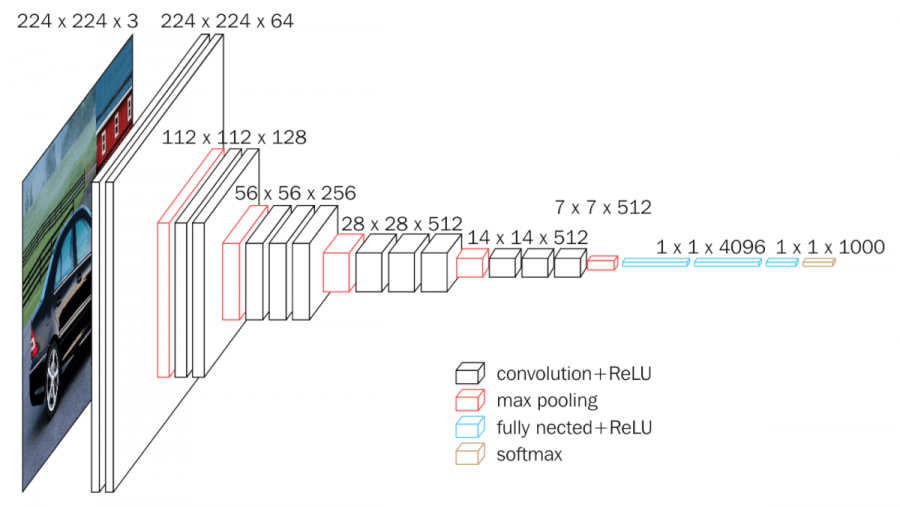
\includegraphics[width=1.0\textwidth]{fig_vgg16_arch.png}
    \caption[VGG16 architecture]{VGG16 architecture.}
    \caption*{Source: \href{https://neurohive.io/en/popular-networks/vgg16}{https://neurohive.io/en/popular-networks/vgg16}}
    \label{fig:vgg16_arch}
    \end{center}
\end{figure}

The VGG16 network architecture is shown in Fig. \ref{fig:vgg16_arch}. The 16 in VGG16 refers to 16 layers that have trainable weights. In VGG16 there are thirteen convolutional layers, five maximum pooling layers, and three dense layers. Each layer in the network is tagged with the dimensions of its output a color that represents its function. Fig. \ref{fig:vgg16_layers_auth} tags the network layers with unique names that we will use to refer to those layers. Convolutional layers are organized in blocks. Layers within a block have the same number of filters.
\begin{figure}[ht]
    \begin{center}       
    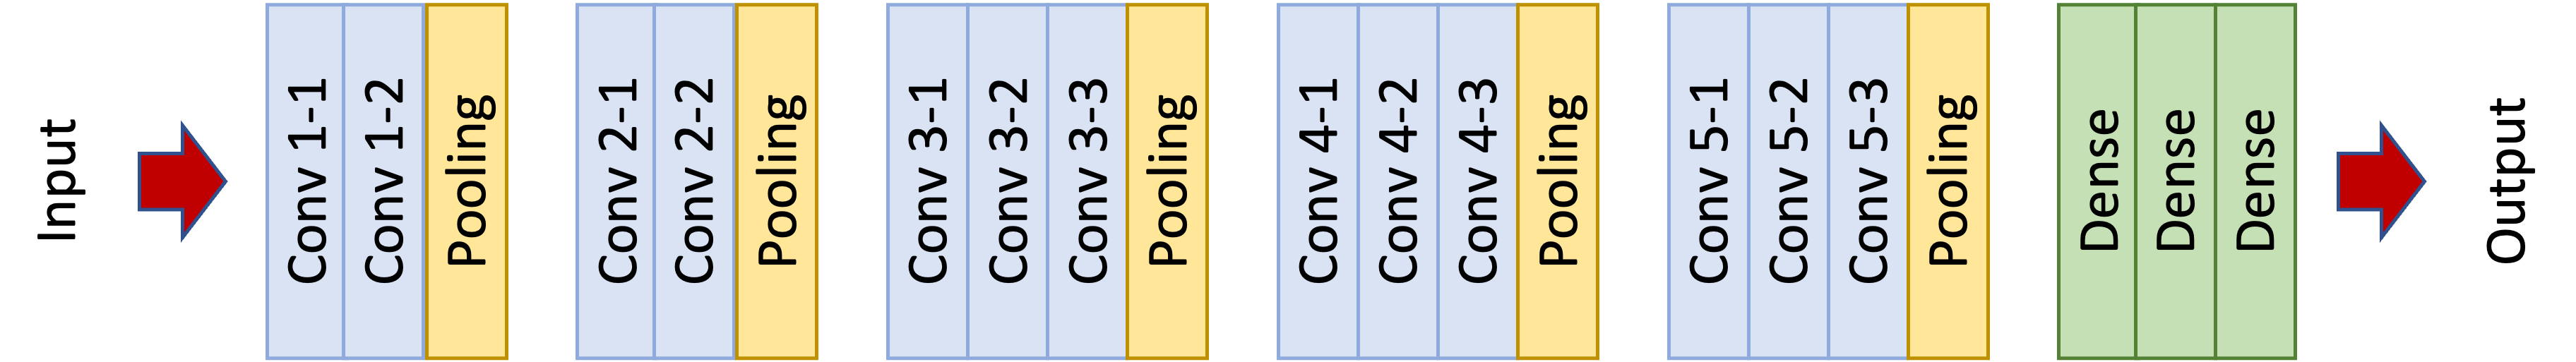
\includegraphics[width=1.0\textwidth]{fig_vgg16_layers_auth.png}
    \caption[VGG16 network layers]{VGG16 network layers.}
    \caption*{Source: Author}
    \label{fig:vgg16_layers_auth}
    \end{center}
\end{figure}

In subsequent sections, we describe the different parts of the architecture.
\subsubsection{Input}
The model expects as input images of fixed size and number of color channels. The dimensions are 224×224x3, standing for width x height x color channels. Typically images in popular datasets (e.g., Imagenet) have different sizes, requiring transformation of the images to resize them to the expected input shape.

\subsubsection{Convolutional layers}
The convolutional layers use a small kernel size of 3×3. A smaller kernel reduces the network’s tendency to over-fit during training. Conv-1 has 2 layers with 64 filters, Conv-2 has 2 layers with 128 filters, Conv-3 has 3 layers with 256 filters, Conv 4 and Conv 5 each have 3 layers with 512 filters. The number of filters represent the output channels of each layer.

\subsubsection{Activation function}
Each convolutional layer is followed by a \acrfull{relu} component. This activation function is a linear function that provides a matching output for positive inputs and outputs zero for negative inputs. The \acrshort{relu} function overcomes the vanishing gradient problem, allowing models to learn faster and perform better. Vanishing gradients occur when more and more layers are used. In this case the gradient can be too small for training to work effectively.

\subsubsection{Pooling layers}
A pooling layer follows a block of convolutional layers with the same kernel size. Pooling helps to reduce the size of the feature maps created by each convolution step. Pooling is given the increase  of the number of filters when going deeper in the network. When the number of filters doubles, also the number of feature maps doubles. The pooling window of 2x2 reduces the size of feature maps by four, keeping computational complexity balanced as we go deeper in the network.

\subsubsection{Fully connected layers}
Three \acrshort{fc} layers follow a stack of convolutional layers: The first two have 4096 channels each, the third performs 1000-way  classification and thus contains 1000 units (one for each class). The final layer is the soft-max layer. This layer ensures that the output values are transformed into confidence scores: Each output value is between 0 and 1 and the total sum of all outputs is 1.

Due to its depth and number of fully-connected nodes, VGG16 has 138 million weights with a storage size over 533MB. This puts high computational and storage requirements on training and storing a model.

\subsection{VGG16-GAP}
Zhou \textit{et al.} \cite{zhou2016cvpr} found that convolutional units to localize objects despite being trained on image-level labels. Despite this fact, this ability is lost when fully-connected layers are used for classification. Zhou \textit{et al.} found that by adding a \acrshort{gap} and tweaking the network, the localization ability of a \acrshort{cnn} can be kept until the final convolutional layer. We refer to this tweaked version of a VGG16 network as the VGG16-GAP network.

Zhou \textit{et al.} found that the localization ability of the network improved when the last convolutional layer before \acrshort{gap} has a higher spatial resolution. Therefore VGG16 is tweaked as illustrated in Fig. \ref{fig:vgg16_gap_layers_auth}. The pooling layer and \acrshort{fc} layers after Conv-5 are removed, resulting in a feature map with resolution 14x14. Then a convolutional layer Conv6-1 is added with kernel size 3×3 and 1024 units, followed by a GAP layer and a softmax layer.
\begin{figure}[ht]
    \begin{center}       
    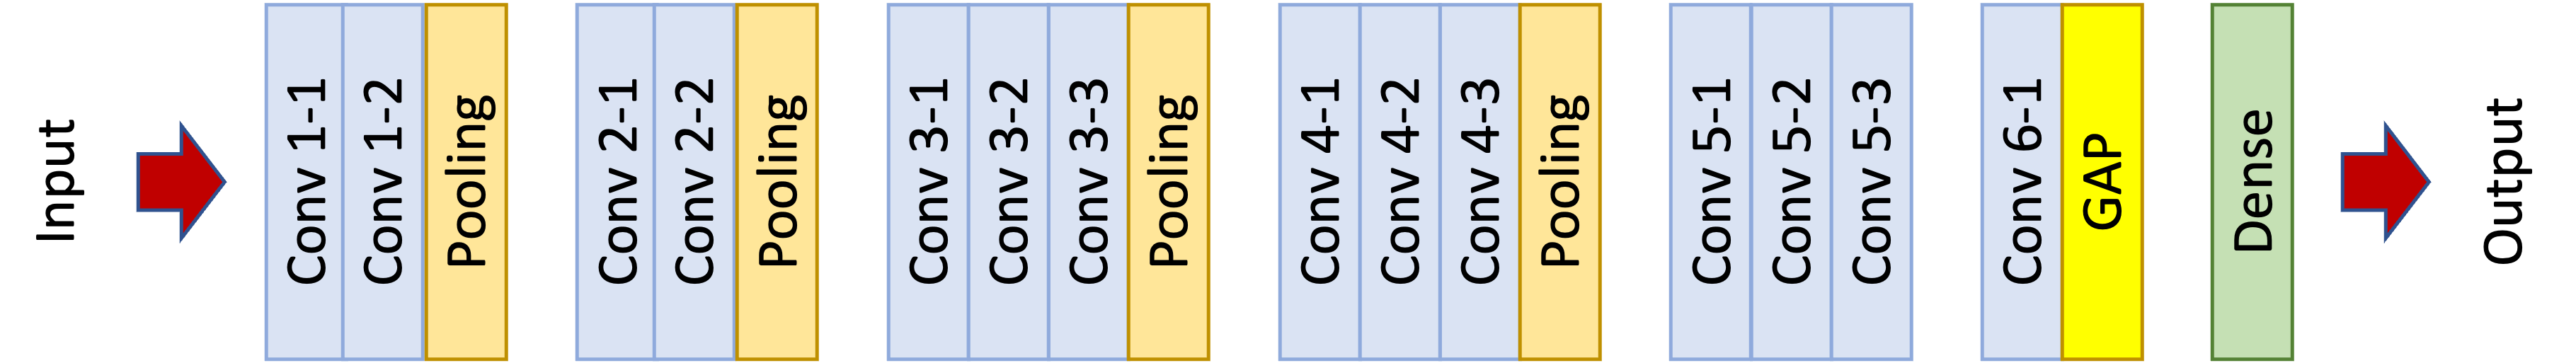
\includegraphics[width=1.0\textwidth]{fig_vgg16_gap_layers_auth.png}
    \caption[VGG16-GAP network layers]{VGG16-GAP network layers.}
    \caption*{Source: Author}
    \label{fig:vgg16_gap_layers_auth}
    \end{center}
\end{figure}

Note that removing fully-connected layers largely decreases network parameters (e.g. 90\% less parameters), but also brings some classification performance drop.

%picture, how it is used and modified for CAM method localization
%parameter count

\subsection{ResNet50 network}
% resaon: Used in MinMaxCAM, more recent than VGG16, efficient (skip 
% explain architecture: deeper networks using skip connections with less parameters connections)
VGG introduced the concept of increasing the number of layers to improve accuracy. However, increasing the number of layers has a negative impact on model convergence. The main reason is the vanishing gradient problem after many layers. This can prevent updating of the model weights during learning.

The ResNet50 architecture was introduced by \cite{he2016deep} and uses the concept of skip connections, allowing inputs to “skip” some convolutional layers. The result is a significant reduction in training time and improved accuracy.

\section{Datasets}
- Why specific datasets, annotations, masks?\\
- Why first with synthetic dataset?\\
\subsection{synthetic dataset}
\begin{itemize}
    \item Propose to use synthetic dataset to limit computational requirements and have control over image structure and ground truth data
    \item describe dataset split (train, val, test), classes, ground-truth, show examples
    \item Better than CIFAR10: cifar 10 too simple, only 10 classes, no background, single instance
    \item Syntehtic dataset inspiration from paper: Quantifying Explainability of Saliency Methods in Deep Neural Networks with a Synthetic Dataset (Erico Tjoa, Guan Cuntai)
\end{itemize}
reason to use synthetic dataset:
\begin{itemize}
    \item Easier to interprete
    \item generate segmentation masks for fine-grained localization evaluation and for datasets with GT segment masks
    \item generate bounding box labels for datasets providing GT bounding box labels
    \item Image size 512x512 large enough for chosen network architectures
    \item generate 4 datasets with different number of object instances per image to measure localization difference.
\end{itemize}

\subsection{ImageNet-1k dataset}
\begin{itemize}
    \item describe dataset split (train, val, test), classes
    \item Why we use imagenet (real, natural images, diverse objects (1000 classes), multi-instance images and GT labels, very popular dataset used in many papers, used in ILSVRC.
\end{itemize}

\section{Learning}
\begin{itemize}
    \item train classification task
    \item approach: training, tuning, pretrained datasets
    \item How we trained our models: SGD, momentum, weight decay, learning rate schedule (step, multistep), regularization (minmaxcam), model weight initialization
    \item stop criterion
\end{itemize}

\section{Localization}
Using CAM WSOL methods to compute attention map. Explain general pipeline from classification, to classification score to feature maps. Principle: features activate on certain characteristics in image that relate to certain class. Feature activations are combined in score maps. Score maps are binarized by threshold. Contours are computed for separate components in cam map. Bounding boxes are computed and compared to ground truth during validation and test to compute localizaton metrics.

Explain selected CAM methods: reason about choice criteria, differences, benefits, limitations
CAM methods: Per cam methode: \\
- Figuur toevoegen \\
- In gewone termen uitleggen wat verschil is \\
- Formules geven en uitleggen (hoe de map gemaakt wordt) \\
Complexity computation \\
- Bezien als evaluatie methode \\
Evaluation metrics \\
- Quantitative evaluation (maxboxaccv3, pxap) \\
- Formules geven en uitleggen \\
- Complexity analysis \\

\subsection{CAM}
CAM: baseline method

\subsection{GradCAM}
GradCAM: Generalization of CAM that doesn’t require a GAP layer in the architecture

\subsection{GradCAM++}

\subsection{ScoreCAM}
ScoreCAM: Shows more focus on object instances. Also seems to do a better job in capturing the features of multiple instances in the explanation map than GradCAM.

\subsection{MinMaxCAM}
MinMaxCAM: regularization of common object regions and background

\section{Evaluation}
\subsection{Computational complexity}
Complexity computation
\begin{itemize}
    \item reasoning about choice between runtime and flops
    \item runtime cpu versus cuda (gpu), synchronization
    \item theoretical versus empirical
\end{itemize}

\subsection{Localization metrics}
\begin{itemize}
    \item Reason about existing versus required metrics
    \item Explain in detail how metrics are computed
    \item MaxBoxAccV3: modified version of MaxBoxAccV2 (Choe et al.,2020b) to support multiple instance WSOL
    \item PxAP (pixel average precision) when ground truth segmentation masks are available.
    \item explain for each method how they capture localization accuracy
    \item explain how localization of small versus large objects are affected by metrics
\end{itemize}

\section{Localization improvement}
Iterative bounding box extraction: Explain intuition for improving localization (see synthetic dataset results and how localization accuracy decreases when number of instances per images increases).

Proposal:
\begin{itemize}
    \item Feed image to model and compute feature activation maps (CAMS)
    \item Extract bounding boxes from binarized CAMS
    \item Mask bounding box areas in image (e.g. with noise, zero values)
    \item Repeat until some stop criterion
\end{itemize}
Variant: Mask image with binarized CAMs.

Possible stop criteria for iterative approach
\begin{itemize}
    \item No new bounding boxes are found
    \item Predefined drop in classification score is reached
    \item Predefined number of iterations is reached.
\end{itemize}

code references:
\begin{itemize}
    \item CAM \cite{code:CAM}
    \item MinMaxCAM \cite{code:MinMaxCAM}
    \item WSOLevaluation\cite{code:WSOLevaluation}
    \item PytorchCAM \cite{code:PytorchCAM}
\end{itemize}